\section{Las c�maras del juego}
\label{s2:sec:camaras}
Como se ha descrito en la secci�n anterior, la interfaz del juego se
encuentra dividida en dos secciones claramente diferenciadas (derecha e
izquierda). Cada secci�n posee sus propios scripts para el dibujado de la
interfaz y el control de las acciones del usuario. Para relacionar ambas
partes, se utiliza un script de nombre \texttt{Director.cs} que se encarga
de comunicarse y coordinar ambas partes.

Para realizar esta divisi�n de la interfaz, se ha decidido utilizar dos
c�maras sobre regiones distintas del espacio, y configurarlas seg�n se
muestra en la figura~\ref{s2:fig:camaras} para que compartan la pantalla.

\begin{figure}[h]
  \begin{minipage}{0.5\textwidth}
    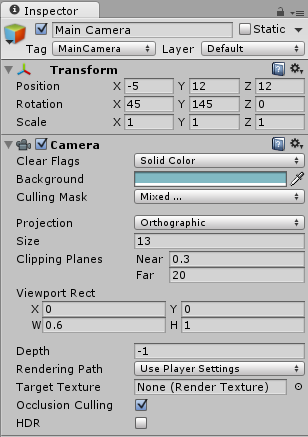
\includegraphics[width=\textwidth]{images/camaras/izq.png}
  \end{minipage}
  \begin{minipage}{0.5\textwidth}
    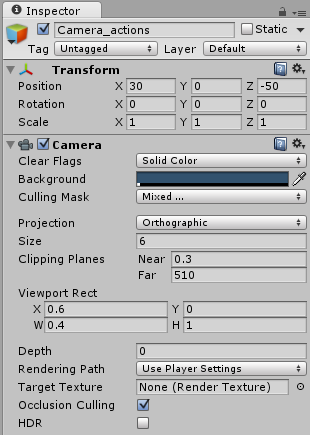
\includegraphics[width=\textwidth]{images/camaras/dcha.png}
  \end{minipage}
  \caption{Configuraci�n de las c�maras}
  \label{s2:fig:camaras}
\end{figure}

Adem�s, para evitar que los textos se rendericen en ambas c�maras, se han
creado dos capas nuevas y configurado el \emph{Culling Mask} de cada c�mara
para que cada una renderice una capa del juego.
